% This is auto-generated file: do not edit!
% Exported from microMathematics Plus, version 2.17.2


This example demonstrates how to
calculate series and integrals.

\subsection{Taylor series}

In mathematics, Taylor series is a
representation of a function as an
infinite sum of terms that are
calculated from the values of the
function's derivatives at a single
point.

For example, Ts(x,N) is the Taylor
expansion as a function of argument x
and the number of terms N:
\begin{center}\begin{tabular}{c}
  $Ts(x,N) := \displaystyle\sum_{n=0}^{N} \frac{{ \left( -1\right) }^{n}}{\left( 2 \cdot n \right)! } \cdot {x}^{2 \cdot n}$
\end{tabular}\end{center}

This expansion approximates the cosine
function:
\begin{center}\begin{tabular}{c}
  $s(x) := cos \left( x\right) $
\end{tabular}\end{center}

If we plot both functions together for
the same interval, they look both
equal:
\begin{center}\begin{tabular}{c}
  $x := \left[ 0,\, 0.1 \,..\, 2 \cdot {\pi} \right]$
\end{tabular}\end{center}
\begin{center}\begin{tabular}{c} 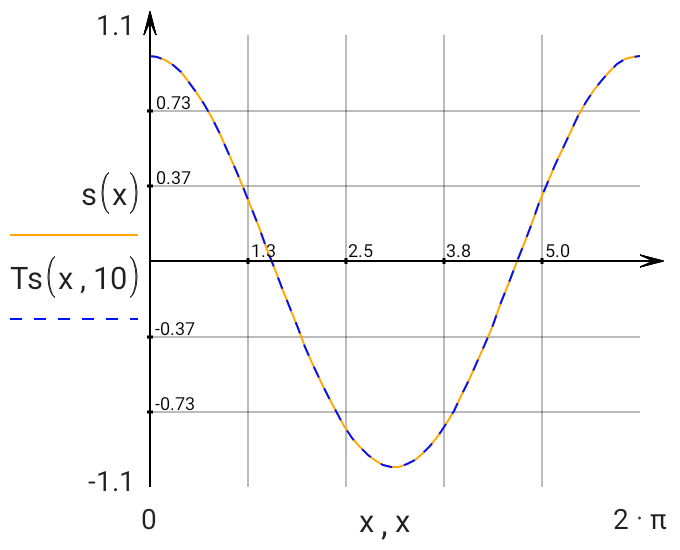
\includegraphics[resolution=320]{graphics/series_and_integrals_fig1.png} \end{tabular}\end{center}

However, there is a numerical error due
to limited number of approximation
terms N. The following function $\Delta$(x,N)
describes this error:
\begin{center}\begin{tabular}{c}
  ${\Delta}(x,N) :=  \left| s \left( x\right)  - Ts \left( x,\, N\right)  \right| $
\end{tabular}\end{center}

We can plot this function in
logarithmic coordinates and see that
the numerical error will be decreased
if we get more terms into the Taylor
summation:
\begin{center}\begin{tabular}{c}
  $N := \left[ 3,\, 4 \,..\, 13 \right]$
\end{tabular}\end{center}
\begin{center}\begin{tabular}{c} 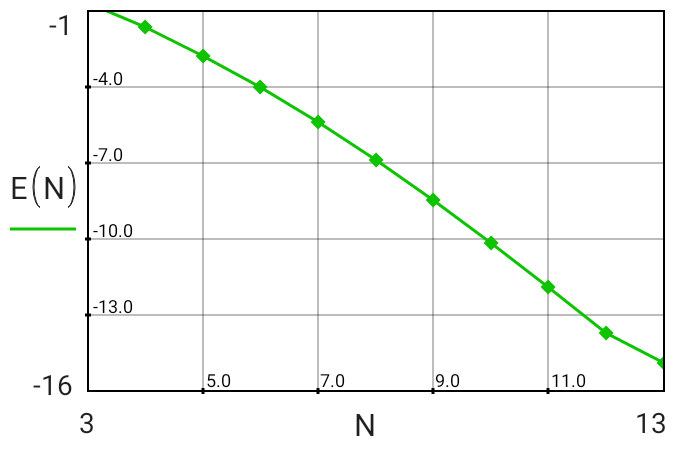
\includegraphics[resolution=320]{graphics/series_and_integrals_fig2.png} \end{tabular}\end{center}

\subsection{Binomial series}

Let us consider this power function:
\begin{center}\begin{tabular}{c}
  $f(x,{\alpha}) := {\left( 1 + x \right)}^{{\alpha}}$
\end{tabular}\end{center}

This function can be approximated using
Binomial series:
\begin{center}\begin{tabular}{c}
  $Tf(x,{\alpha},N) := \displaystyle\sum_{n=0}^{N}  \left( \displaystyle\prod_{k=1}^{n} \frac{{\alpha} - k + 1}{k}\right)  \cdot {x}^{n}$
\end{tabular}\end{center}

We can also plot both functions (the
given power function and its
approximation) together on the same
plot:
\begin{center}\begin{tabular}{c} 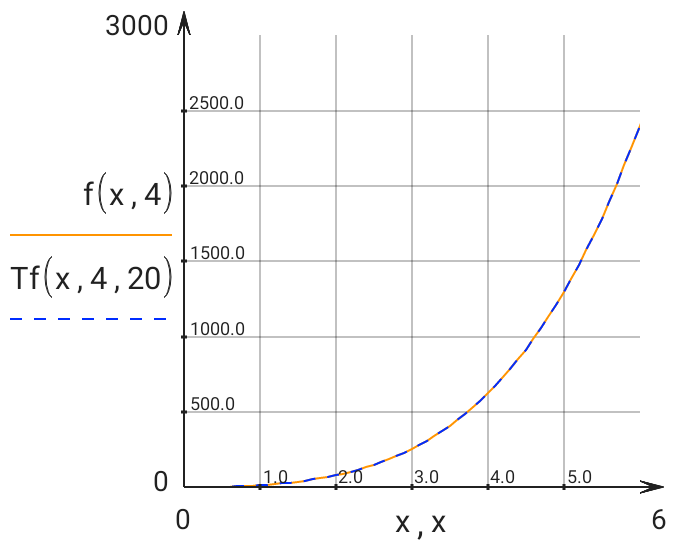
\includegraphics[resolution=320]{graphics/series_and_integrals_fig3.png} \end{tabular}\end{center}

\subsection{Integrals}

It is also possible to calculate a
definite integral numerically using
Simpson method. For example, we can
calculate the integral using ''Result
View'' element:
\begin{center}\begin{tabular}{c}
  $\displaystyle\int_{0}^{3 \cdot pi / 2}{cos \left( \frac{2 \cdot x}{9}\right) }^{-2}\, dx = 7.79423$
\end{tabular}\end{center}

The analytical solution is
\begin{center}\begin{tabular}{ccc}
  $I := \frac{9 \cdot \sqrt{3} }{2}$ &
  ,    &
  $I = 7.79423$ \cr
\end{tabular}\end{center}

Numerical error can be calculated as:
\begin{center}\begin{tabular}{c}
  $\displaystyle\int_{0}^{3 \cdot pi / 2}{cos \left( \frac{2 \cdot x}{9}\right) }^{-2}\, dx - I = 4.26681E-9$
\end{tabular}\end{center}

This error depends on the value
''Significant digits in result'' that
can be changed in the ''Document
Settings'' dialog available from the
action bar:
\begin{center}\begin{tabular}{c} 
\includegraphics[resolution=320]{graphics/series_and_integrals_fig4.png} \end{tabular}\end{center}

If this value increased, the threshold
that controls the Simpson method
precision will also be increased.